\ylDisplay{Kontuuri takistus} % Ülesande nimi
{Koit Timpmann} % Autor
{lõppvoor} % Voor
{2019} % Aasta
{P 7} % Ülesande nr.
{3} % Raskustase
{
% Teema: Elektriõpetus

\ifStatement
Kõrvaloleval joonisel esitatud kujund on valmistatud ühesugusest traadist. Kujundi diameetri pikkuse traadijupi elektriline takistus $R = 1$ $\Omega$. Kui suur on vooltugevus kujundi diameetris $AC$, kui pinge punktide $A$ ja $B$ vahel $U = 1,5$ $V$. 
\begin{center}
	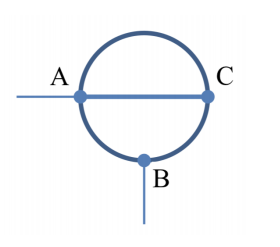
\includegraphics[width=0.5\linewidth]{2019-v3p-07-yl.png}
\end{center}
\fi

\ifHint
Vooluahela paremaks mõistmiseks on mõistlik kujutada elektriskeem erinevate takistite rööp- ja jadaühendusskeemina.
\fi

\ifSolution
Diagonaali takistus on $R_{diagonaal} = 1$ $\Omega$.
Kuna ringi ümbermõõt $c = \pi d$ ja $R_{AC}$ võrdub poolega ringi ümbermõõdust, siis $R_{AC} = 1,57$ $\Omega$.
$R_{AB}$ ja $R_{CB}$ on mõlemad veerand ringi ümbermõõtu, seega $R_{AB} = R_{CB} = 0,785$ $\Omega$.
Leiame vooluringi kogutakistuse. Takistid $R_{AC}$ ja $R_{diameeter}$ on rööbiti ühendatud, seega nende kogutakistus on:
$R_{roop} = \frac{1}{R_{AC}} + \frac{1}{R_{diameeter}} = 0,61$ $\Omega$.
Nendega on jadamisi ühendatud tekisti $R_{CB}$. Takistite jada takistus $R_{jada} = 0,61 \Omega + 0,785 \Omega = 1,395 \Omega$.
Jadasse on ühendatud takistitega on omakorda rööbiti ühendatud takisti $R_{AB}$. Seega, vooluringi kogutakistus tuleb $R = 0,5$ $\Omega$.

Arvutame kogu voolutugevuse. Ohmi seadusest saame, et 
$I = \frac{U}{R} = 3$ $A$.
Kuna takisti $R_{AB}$ kujutab endast vooluringi ühte haru, siis selle takisti otstel on pinge $1,5$ $V$ ja voolutugevus takisitis on $I_{AB} = \frac{1,5V}{0,785 \Omega} = 1,91$ $A$.
Seega, vooluringi teises harus on voolutugevus 
$I_{ulemine} = I - I_{AB} = 1,09$ $A$.
Pingelang takistil $R_{CB}$ võrdub $U_{CB} = I_{ulemine} \cdot R_{CB} = 0,856 $ $V$.
Pinge otsitaval takistil on võrdne $U_{diameeter} = u- U_{CB} = 0,644$ $V$ ja voolutugevus diagonaalis on võrdne
$I_{diameeter} = \frac{0,644V}{1 \Omega} = 0,64$ $A$
\begin{center}
	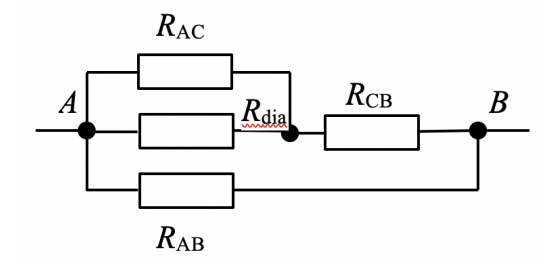
\includegraphics[width=0.5\linewidth]{2019-v3p-07-lah.png}
\end{center}
\fi
}